%! Author = chtompki
%! Date = 1/14/26
\documentclass[12pt]{amsart}
% Default margins are too wide all the way around. I reset them here
\setlength{\hoffset}{-.75in}
\setlength{\textwidth}{6.5in}
\setlength{\voffset}{-.5in}
\setlength{\textheight}{9.0in}
\usepackage{amsmath}
\usepackage{amssymb}
\usepackage{amsthm}
\usepackage{enumitem}
\usepackage{setspace}
\usepackage{graphicx}

\newenvironment{solution}
{\begin{proof}[Solution]}
{\end{proof}}

\NewDocumentCommand{\vitem}{v}{%
    \item[\texttt{#1}]%
}

\title{Numerical Analysis\\Problem Set 1}
\author{Rob Tompkins}
\date{\today}

\begin{document}
    \maketitle
    \date{\today}
    \begin{onehalfspace}
        We begin by noting that all of the files referenced in this document are available at:
        \underline{https://github.com/chtompki/MathSpring2026/tree/main/NumericalAnalysis/ProblemSet1}
        % Problem 1
        \textbf{1.} The value of $\pi$ is given by the alternating series:
        \begin{displaymath}
            \pi = 4 \sum_{n=0}^{\infty} \frac{(-1)^n}{2n+1}
            = 4 \left(1 - \frac{1}{3} + \frac{1}{5} - \frac{1}{7}+ \cdots\right)
        \end{displaymath}

        (a) Use this series to construct an algorithm to approximate the value of $\pi$ to within a specified
        tolerance, $\varepsilon$. The algorithm should be general to allow for any $\varepsilon$. Provide a theoretical
        upperbound $\epsilon$ on the error of your approximation. \underline{Hint.} It may be useful to recall known
        properties of the partial sums of alternating series.

        (b) Run your algorithm with a tolerance value of $\varepsilon = 5\times 10^{-3}$ and show that your result is
        within $\varepsilon$ of $\pi = 3.1415926\ldots$

        (c) Make a plot of $\varepsilon$ versus the number $N$ of reuired terms in your algorithm on a log-log scale.
        What is the slope of the line that the resulting plot approaches a $N$ increases? Plot the actual error as a
        function of $N$ on the same axes, you may treat the stored value of $\pi$ as ``exact.'' How does the actual
        error compare to the estimated threshold?
        \begin{solution}
            (a) Our algorithm is given in the file ``problem1.m'' but also below as it is simple:
            \begin{verbatim}
                function approximatePi = computePiPlotError(error)
                    p = 0;
                    sum = 0;
                    index = 0;
                    pApproximated = [];
                    indexedError = [];
                    while (abs(pi - p) > error)
                        sum = sum + (-1)^index * 1/(2*index + 1);
                        p = 4*sum;
                        index = index + 1;
                        pApproximated(index) = p;
                        err = abs(pi - p);
                        indexedError(index) = err;
                    end
                    approximatePi = p;
                    loglog(1:index,indexedError,'--k')
                    xlabel('Iteration Index n');
                    ylabel('Error');
                    title('Error in Pi Approximation');
                end


                format long
                approx_pi = computePiPlotError(5e-3)
                pi - approx_pi
            \end{verbatim}
            Note, an upper bound on $\varepsilon$ should be $|pi - 4| \approx 0.85840$.

            (b) When we run this function we get the following output from matlab:
            \begin{align*}
                p &= 3.136592684838816 \\
                \varepsilon &= 0.004999968750977
            \end{align*}

            (c) When we plot $\varepsilon$ versus the number of iterations of our algorithm to try to find $\pi$ we
            get:
            \begin{figure}[!ht]
                \centering
                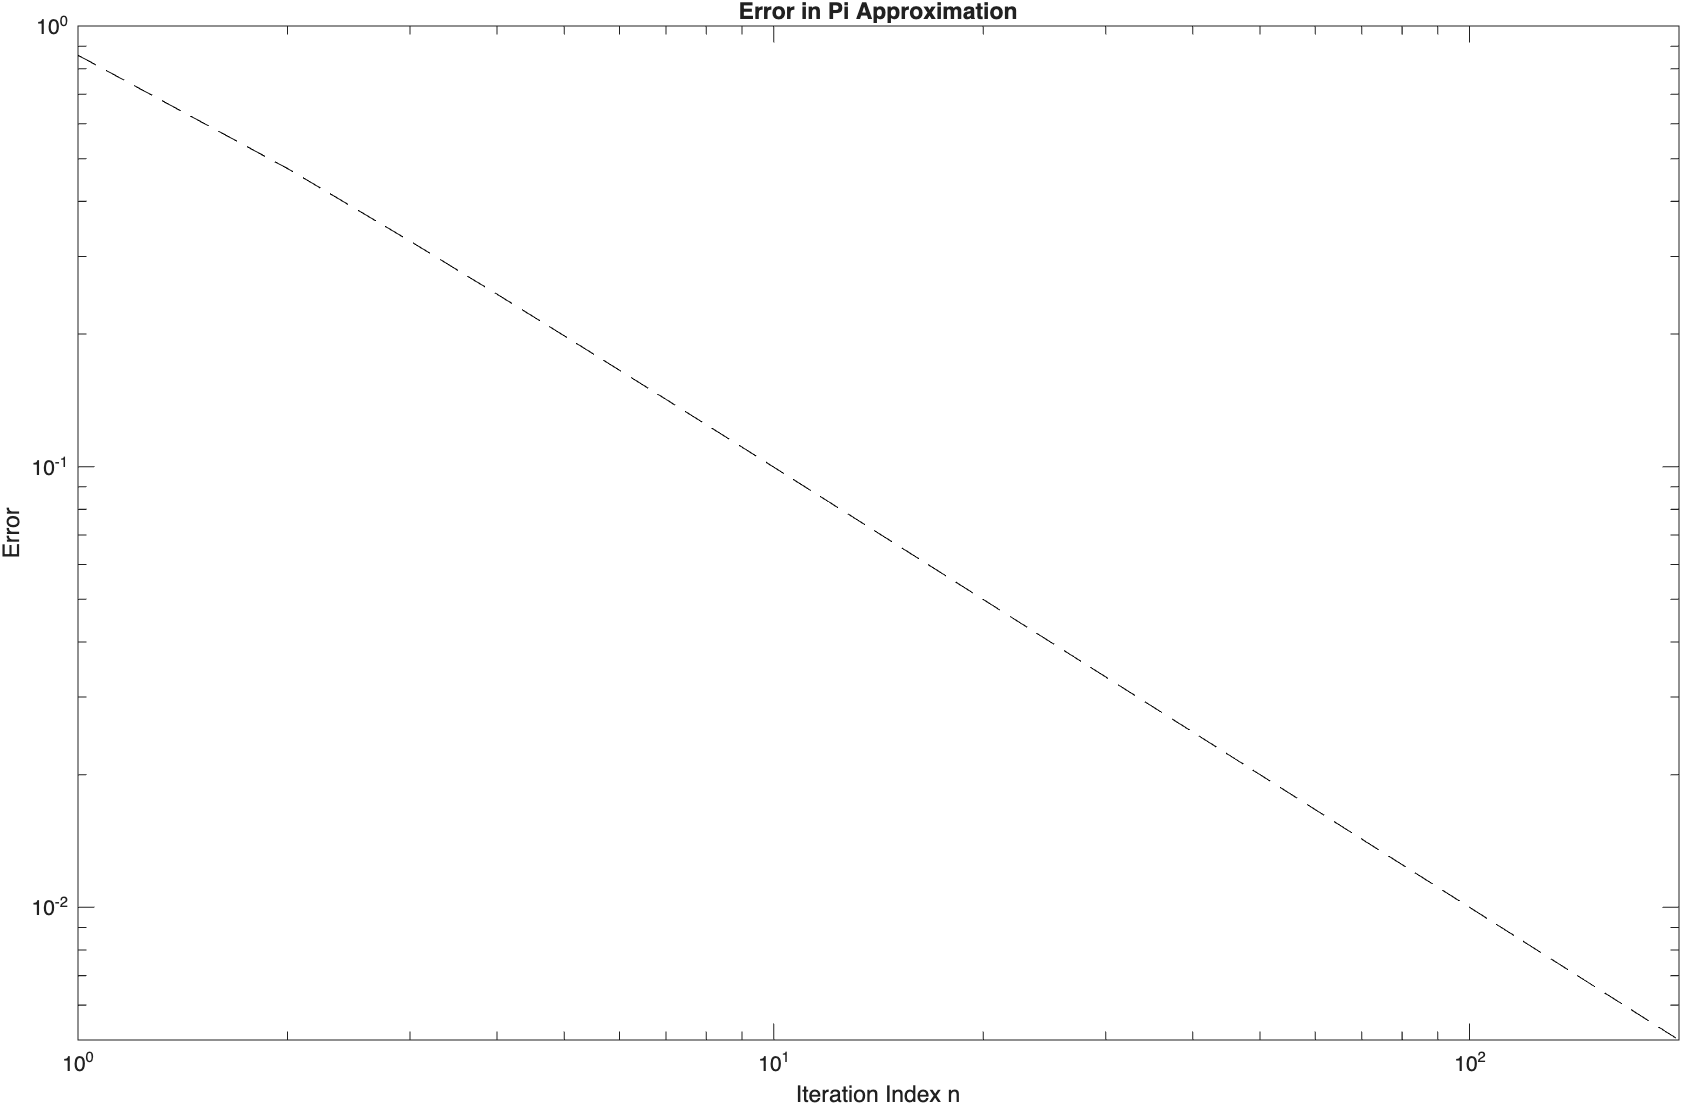
\includegraphics[scale=0.4]{Problem_1_Figure.png}
                \caption{Log-Log plot $\varepsilon$ versus $N$}
            \end{figure}
            I'm not exactly sure what we're going for here with the ``actual error''. The only thing that I can come up
            with is considering the remainder of the tail of the summation after the $n^{\text{th}}$ iteration.
            \begin{displaymath}
                \text{err}^{\text{actual}}_n = 4 \sum_{k = n + 1}^{\infty} \frac{(-1)(^k)}{2k + 1}
            \end{displaymath}
            I suppose we could pick some huge $k$, say $10^{12}$ and iterate from our curren $n$ to there to get the
            actual error. But to do so I would end up using the symbolic computation capabilities in matlab.
            I've added a ``problem1b.m'' in the directory but the computational capacity on the ``symsum'' function
            is insufficient for the problem.

        \end{solution}

        % Problem 2
        \textbf{2.} Numerically determine which of the following limits approaches 1 faster. Then confirm the
        numerical evidence by determining the rate of convergences of each sequence
        \begin{displaymath}
            \lim_{n\rightarrow 0}\frac{\sin(x^2)}{x^2}\qquad\text{versus}\qquad\lim_{n\rightarrow 0}\frac{(\sin x)^2}{x^2}.
        \end{displaymath}
        \begin{solution}
            We'll just run a table here for $\{10^0, 10^{-1}, 10^{-2},\ldots,10^{-9}\}$ to look at convergence of the
            functions listed above. The code for this problem is minimal command line work using vectors with the scalar
            versions of the $\sin$ and arithmatic functions. \\

            \centering
            \begin{tabular}{ccc}
                $n$ & $\sin(x^2)/x^2$ & $(\sin x)^2/x^2$ \\
                \hline
                $10^0$    & -0.005063656411098 & 0.002959589690933 \\
                $10^{-1}$ & 0.841470984807897 & 0.708073418273571 \\
                $10^{-2}$ & 0.999983333416666 & 0.996671107937918 \\
                $10^{-3}$ & 0.999999998333333 & 0.999966667111108 \\
                $10^{-4}$ & 0.999999999999833 & 0.999999666666711 \\
                $10^{-5}$ & 1.000000000000000 & 0.999999996666667 \\
                $10^{-6}$ & 1.000000000000000 & 0.999999999966667 \\
                $10^{-7}$ & 1.000000000000000 & 0.999999999999667 \\
                $10^{-8}$ & 1.000000000000000 & 0.999999999999997 \\
                $10^{-9}$ & 1.000000000000000 & 1.000000000000000
            \end{tabular}

            Now as to find the rate of convergence for the functions, we'll consider them one at a time.
            For $\sin(x^2)/x^2$ notice that
            \begin{displaymath}
                \frac{\sin(x^2)}{x^2} \le \frac{1}{x^2}
            \end{displaymath}
            So our rate of convergence is $\mathcal{O}(1/x^2)$.

            For $(\sin x)^2/x^2$ we first notice that
            \begin{displaymath}
                \lim_{x\rightarrow 0} \frac{\sin(x)}{x} = 1
            \end{displaymath}
            Therefore, we see that
            \begin{displaymath}
                \lim_{x\rightarrow 0} \frac{(\sin x)^2}{x^2} = \left( \lim_{x\rightarrow 0} \frac{\sin(x)}{x}\right)^2 = 1^2 = 1
            \end{displaymath}
            and our convergence is on the order of $\mathcal{O}(1/x)$.

        \end{solution}

        % Problem 3
        \textbf{3.} (a) Consider the function $f_c(x) = x^2 -12x + c$. What are the zeros of $f_c$ with $c = 35$? What
        are the zeros of $f_c$ with the slight constant shift $c = 35 - 10^{-2}$? Relative to the size of change in
        the constant term $c$, how big is the change in the zeros of the function?

        (b) consider the function $g_c(x) = x^2 - 10x + c$. What are the zeros of $g_c$ with $c = 25$? What are the
        zeros of $g_c$ with the slightest constant shift $c = 25 - 10^{-2}$? Relative to the size of change in the
        constant term, how big is the change in the zeros of the function?

        (c) Compare the nature of the roots of $f$ and $g$. How might this contribute to the relative changes in the
        zeros for each function?
        \begin{solution}
            (a) Using the quadratic formula we quikcly see that:
            \begin{displaymath}
                x_a = \frac{12 \pm \sqrt{144 - 4(35)}}{2} = \{7, 5\}
            \end{displaymath}
            but if we let $c = 35-10^2$, our zeros become (using matlab for the calculation):
            \begin{displaymath}
                x_b = \frac{12 \pm \sqrt{144 - 4(35)}}{2} = \{7.048808848170152,4.951191151829848\}
            \end{displaymath}
            and we note that the values came from the opposing fomulae. The shift in the zero is $x_a - x_b$ which
            follows as
            \begin{displaymath}
                x_a - x_b = \{0.048808848170152,0.048808848170152\}.
            \end{displaymath}

            (b) Similarly to (a) we use the quadratic formula to quickly see that we have a singular root at:
            \begin{displaymath}
                x_a = \frac{10\pm\sqrt{100 - 4(25)}}{2} = 5
            \end{displaymath}
            However, if we let $c = 25-10^{-2}$, we get the following:
            \begin{displaymath}
                x_b = \frac{10\pm\sqrt{100 - 4(25-10^{-2})}}{2} = \{5.316227766016840, 4.683772233983160\}
            \end{displaymath}
            The shift in zero is $x_a - x_b = 0.316227766016840$.

            (c) The nature of the roots differ from $f$ and $g$ in that $g$ is tangent to the $x$ axis at $5$, where
            as $f$ has two distinct roots at $c = 35$, $5$ and $7$.
        \end{solution}

        % Problem 4
        \textbf{4.} Identify the potential roundoff error problems in the following algorithm for calculating
        the roots of the quadratic equation $ax^2 + bx + c = 0$.
        \begin{itemize}[label={}]
            \centering
            \vitem{GIVEN:} real coefficients $a, b, c$
            \vitem{STEP 1:} calculate $disc = \sqrt{b^2 - 4ac}$
            \vitem{STEP 2:} calculate $root1 = -2c/(b + disc)$
            \vitem{STEP 3:} calculate $root2 = (-b/a) - root1$
            \vitem{OUTPUT:} $root1$ and $root2$
        \end{itemize}
        Note that this algorithm uses the fact that the sum of the roots of $ax^2 + bx + c = 0$ is equal to $-b/a$.
        \begin{solution}
            If we're considering all the possibilities for roundoff error, we start by noticing that we initially
            have the possibility for roundoff error in that the coefficients $a, b, c$ may infact be irrational needing
            to be initially rounded.

            In $\texttt{STEP 1}$ we can have rounding problems when $b^2\approx 4ac$ by subtracting numbers
            that are nearly identical.

            In $\texttt{STEP 2}$ we can have real problems when $b+ disc\approx 0$ because the denominator has
            large relative error.
            $root1$ in this case becomes highly inaccurate and may overflow. Also if $c$ is tiny $-2c$ could underflow.

            In $\texttt{STEP 3}$ if we are dealing with subtraction of nearly equal numbers then we could have
            roundoff error. The cases when this could occur would be if the roots are of vary different magnitudes
            and the large one is $root1$.
            Lastly notice that if $a$ is tiny, $-b/a$ can overflow.
        \end{solution}

        % Problem 5
        \textbf{5.} (a) Plot the function $f(x) = \text{ln}(1+ x) - \cos(x) - x + 1$ over the interval
        $-5\times 10^{-6}\le x\le 5\times10^{6}$ using 1001 uniformly spaced points in $x$.

        (b) Reformulate $f$ to avoid the cancellation error, and then repeat part (a).

        (c) Describe the issues with the original formulation in part (a) and how they were resolved with the
        reformulation in part (b).
        \begin{solution}
            (a) Running the plot using this order of operations yields the plot in Figure 2.
            \begin{figure}[!ht]
                \centering
                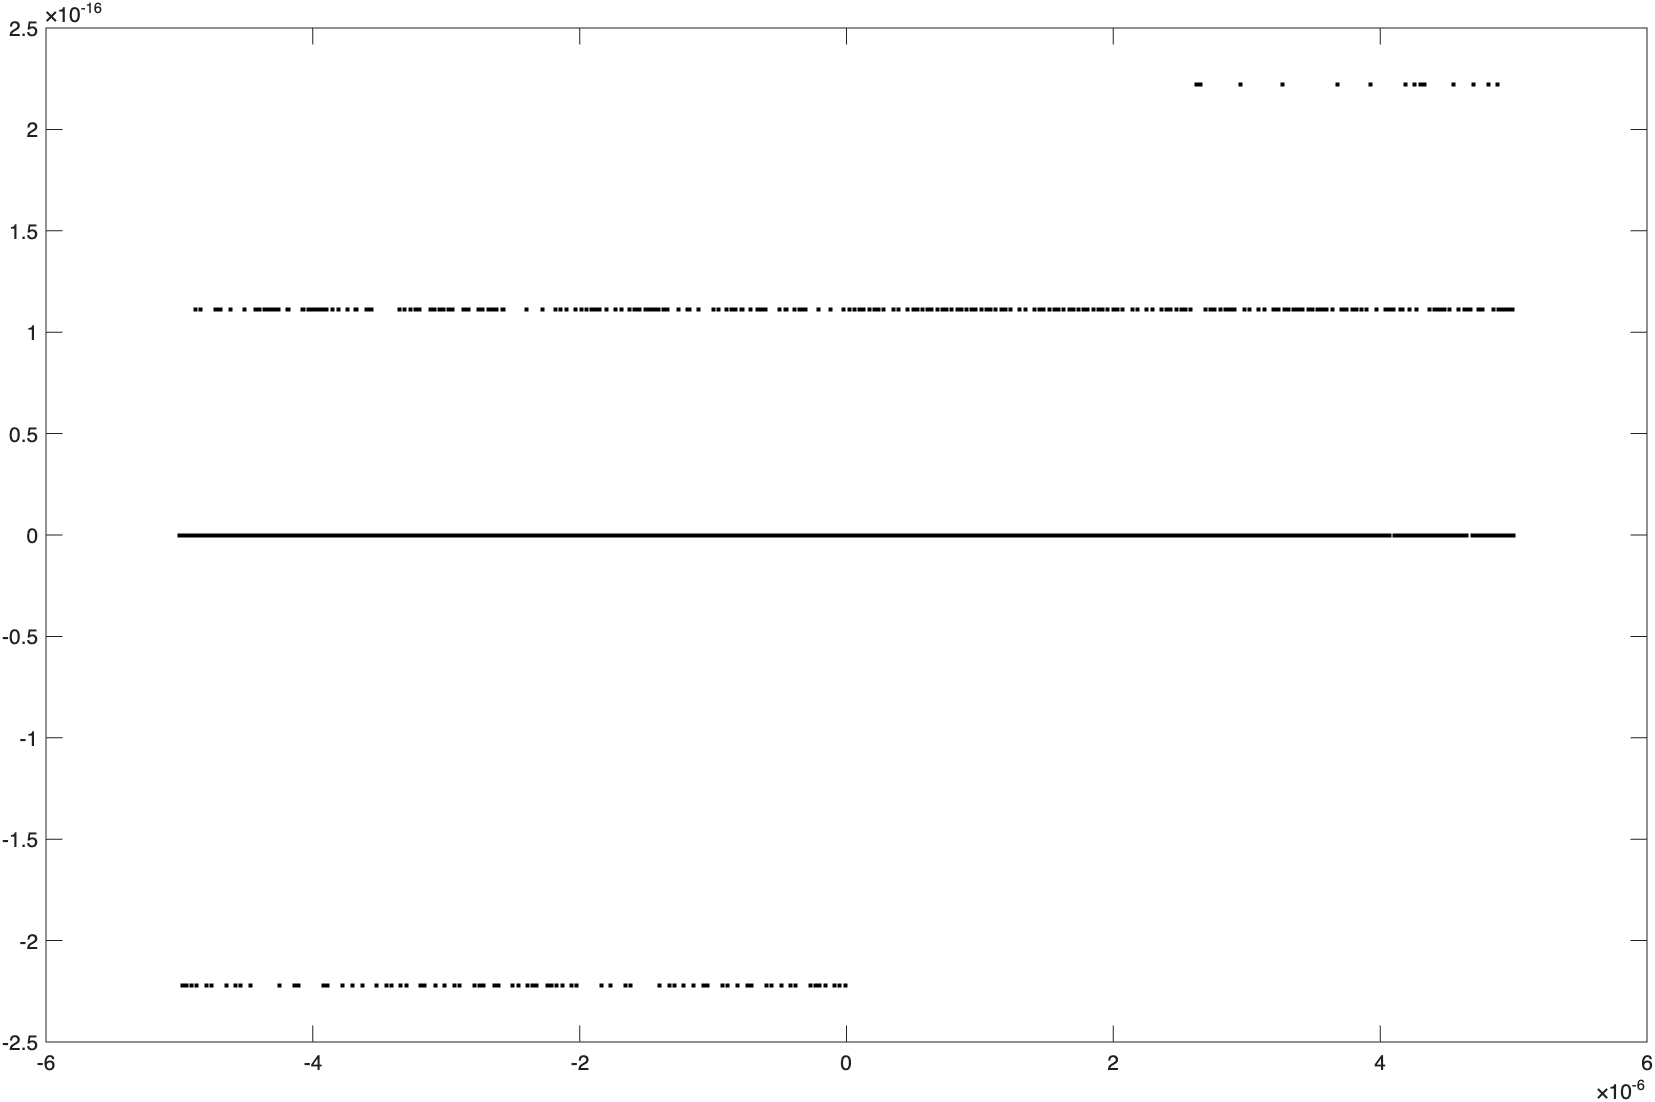
\includegraphics[scale=0.4]{Problem_5_Figure_1.png}
                \caption{Plot of $\text{ln}(1+ x) - \cos(x) - x + 1$ using 1001 uniformly spaced points over the range}
            \end{figure}

            (b) If we simply rearrange the function to put the additions and subtractions in a different order, for example
            \begin{displaymath}
                f(x) = (\text{ln}(1+x) - x) + (1 - \cos(x))
            \end{displaymath}
            we get the graph in Figure 3, which we overlayed on top of part (a).
            \begin{figure}[!ht]
                \centering
                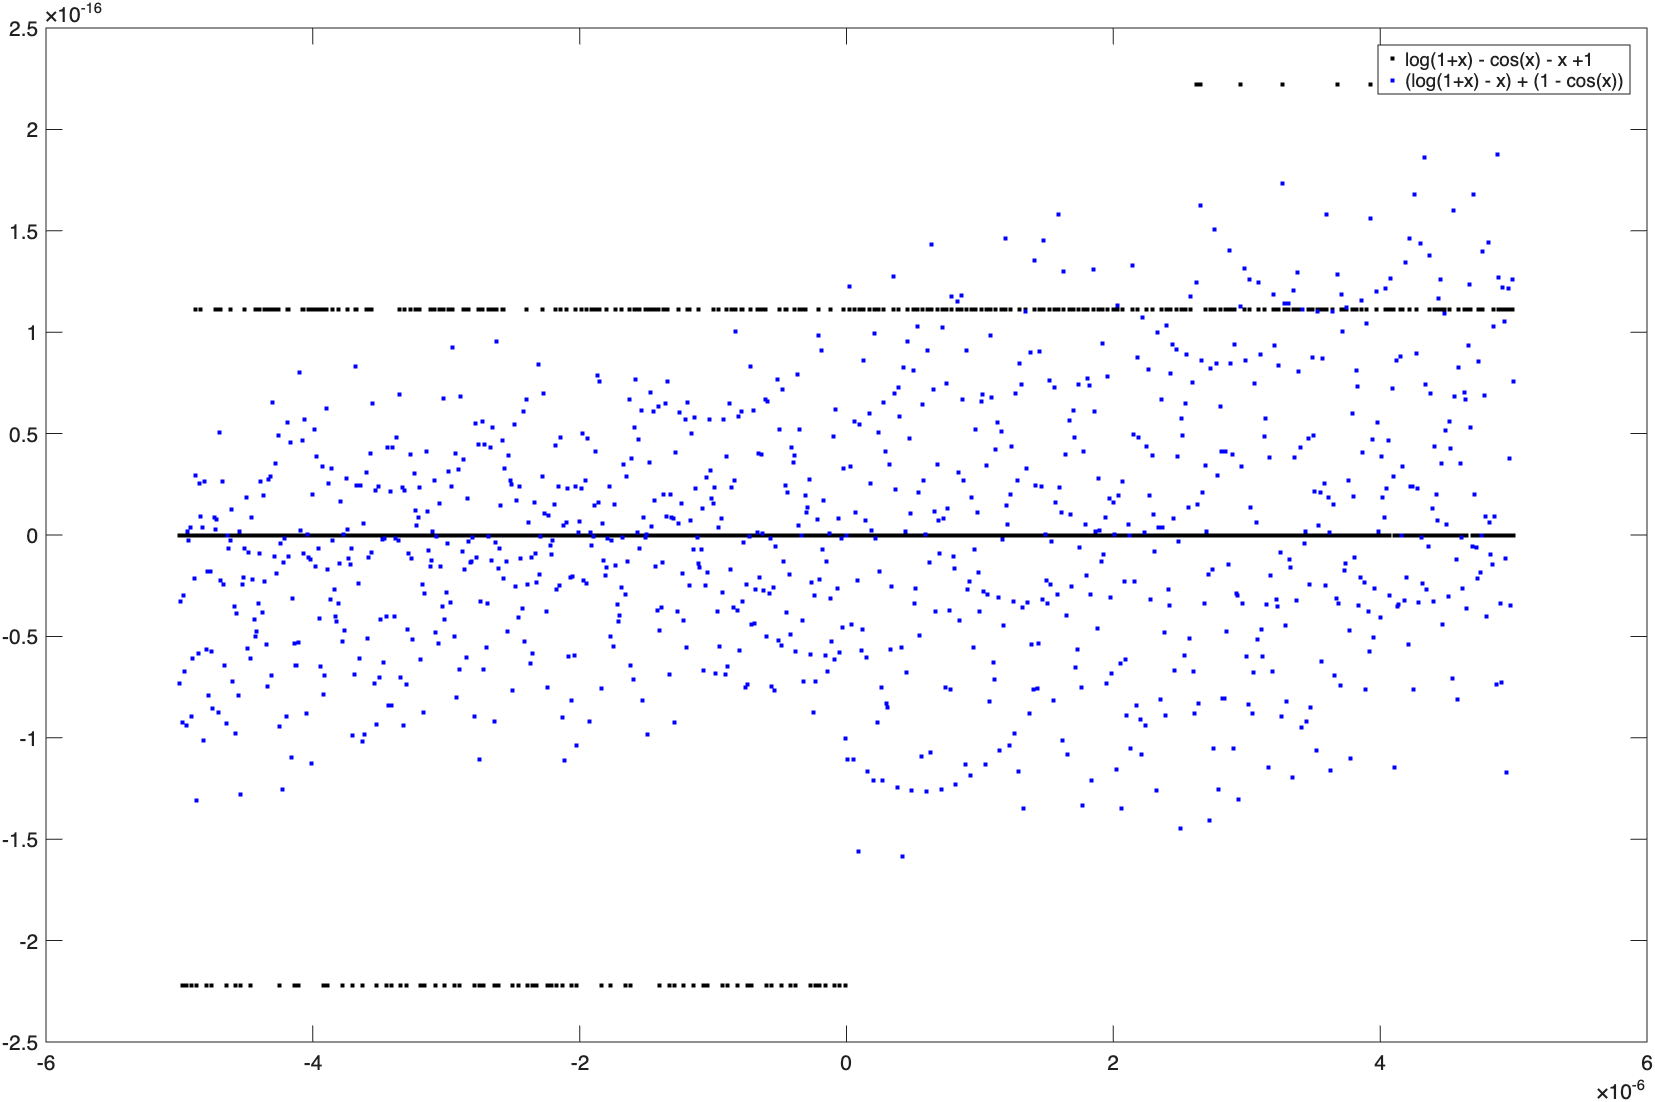
\includegraphics[scale=0.4]{Problem_5_Figure_2.png}
                \caption{Plot of $\text{ln}(1+ x) - \cos(x) - x + 1$ versus $(\text{ln}(1+x) - x) + (1 - \cos(x))$}
            \end{figure}

            (c) The main issue with the problem stemmed from roundoff error around the subtraction between $\cos(x)$
            and $x$ because we're so close to 0.
            So that essentially forces us into buckets as we see in the plot in Figure 2.
        \end{solution}


        % Problem 6
        \textbf{6.} (a) Determine the third-degree Taylor polynomial associated remainder term for the function
        $f(x) = \sqrt(1 + x)$. Use $x_0 = 0$.

        (b) Using the result of part (a), approximate $\sqrt{1.5}$, and compute the theoretical error bound
        associated with this approximation. Compare the theoretical error bound with the actual error.

        (c) Compute the following limit and determine the corresponding rate of convergence:
        \begin{displaymath}
            \lim_{x\rightarrow 0} \frac{\sqrt{1+x} - 1 - \frac{1}{2}x}{x^2}
        \end{displaymath}
        \begin{solution}
            Problem 6
        \end{solution}

        % Problem 7
        \textbf{7.} Consider the linear system $Ax=b$ with $A=\left[\begin{matrix}3.4 & 2.8 \\ 8.0 & 6.6\end{matrix}\right]$,
        $x = \left[\begin{matrix}x_1 \\ x_2\end{matrix}\right]$, and $b = \left[\begin{matrix}3.4 \\ 8.0\end{matrix}\right]$.

        (a) Determine the analytic solution by hand. (How do we know that it is unique, i.e. that the problem is well-posed?)

        (b) Now solve the system with $b = \left[\begin{matrix}3.41 \\ 8.0\end{matrix}\right]$. You may use your computer.

        (c) Given the difference in solutions for parts (a) and (b), comment on the conditioning of the problem. What is
        $\text{det}[A]$ and for what values with the problem be ill-posed?
        \begin{solution}
            Problem 7
        \end{solution}
    \end{onehalfspace}
\end{document}